\section{Ứng dụng các cơ chế tiến hóa trong tối ưu} % (fold)
\label{sec:Ứng dụng các cơ chế tiến hóa trong tối ưu}

\subsection{Chọn lọc tự nhiên và Thuyết tiến hóa của C. Darwin} % (fold)
\label{sub:Chọn lọc tự nhiên và Thuyết tiến hóa của C. Darwin}

\begin{frame}{Chọn lọc tự nhiên và Thuyết tiến hóa của C. Darwin}
Gần 4 tỉ năm trước, sự sống xuất hiện trên Trái Đất. Sau một khoảng thời gian
ấy, sự sống đã len lỏi đến mọi ngóc ngách của địa cầu, mang đủ loại hình thù từ
đơn giản đến phức tạp. Các nhà sinh học, sau khi nhìn thấy sự đa dạng này, đặt
ra câu hỏi rằng: tại sao các quy luật của tự nhiên, dường như ưa thích sự hỗn
loạn và thiếu trật tự, lại có thể tạo ra những loại tổ chức vật chất phức tạp và
dường như có chủ ý này.

Cho đến ngày nay, câu hỏi này vẫn chưa có một lời giải thích thỏa đáng. Tuy
nhiên, \textbf{Thuyết Tiến hóa} của C. Darwin đã, mặc dù có nhiều lỗ hổng, đã
trả lời được câu hỏi này một cách tương đối hoàn thiện.
\end{frame}

\begin{frame}{Chọn lọc tự nhiên và Thuyết tiến hóa của C. Darwin}
\begin{figure}
  \centering
  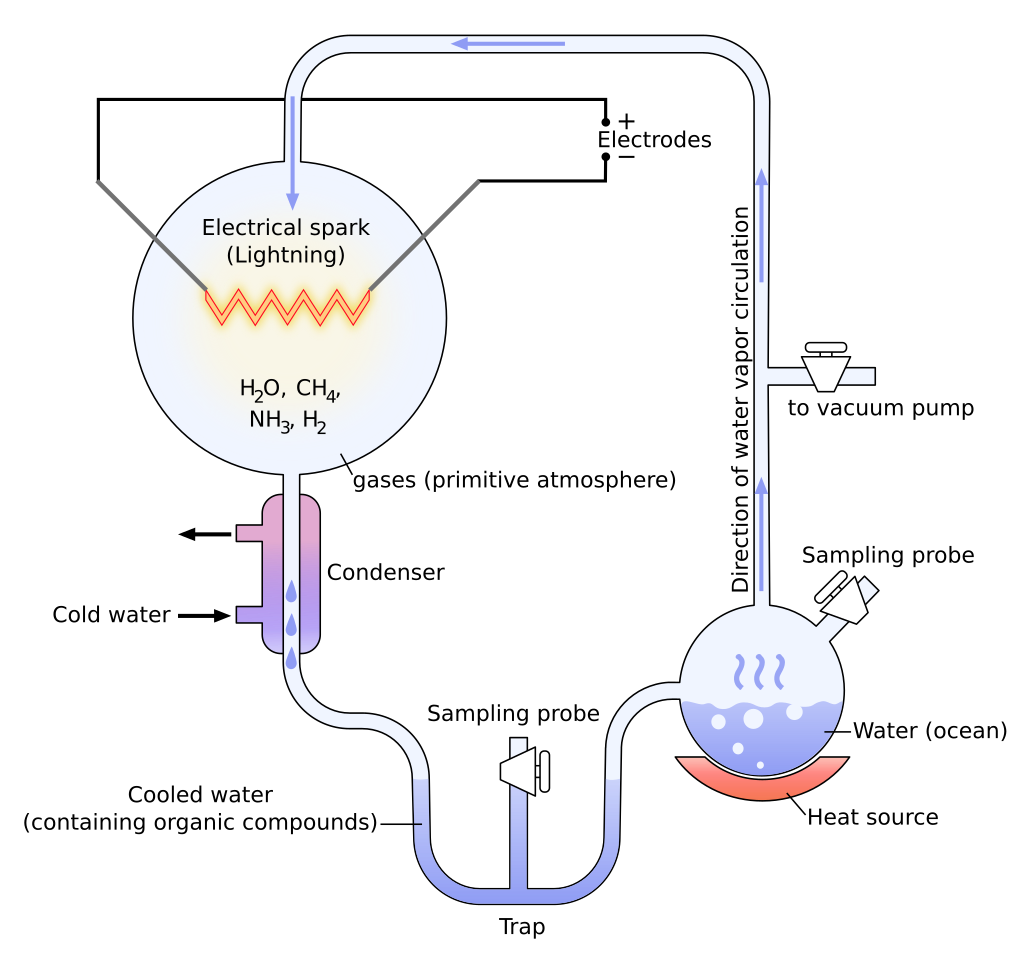
\includegraphics[width=0.8\textwidth, height=0.7\textheight,
  keepaspectratio]{res/miller-urey.png}
\captionsetup{justification=centering,margin=3cm}
  \caption{Thí nghiệm Miller-Urey, một thí nghiệm thất bại trong việc giải thích nguồn
  gốc của sự sống.}
\end{figure}
\end{frame}

\begin{frame}{Chọn lọc tự nhiên và Thuyết tiến hóa của C. Darwin}
Thuyết tiến hóa của C. Darwin đề cao một quá trình xảy ra trong tự nhiên:
\textbf{Chọn lọc tự nhiên}, coi đây là yếu tố quan trọng nhất sản sinh ra mọi
loài sinh vật.

Theo C. Darwin, để chọn lọc tự nhiên hoạt động như những gì xảy ra trong thực tế,
cần có ba điều kiện sau:

\begin{itemize}
\item Tính kế thừa (Heredity): Cần có một cách nào đó để chuyển giao các tính
  trạng từ cá thể cha mẹ sang các cá thể đời con.
\item Tính đa dạng (Variation): Trong hệ sinh thái, các cá thể cần có nhiều đặc
  điểm khác nhau, hoặc một cách để tạo ra các cá thể biến thể có đặc điểm khác
  với quần thể.
\item Tính chọn lọc (Selection): Phải có một phương thức nào đó mà một số cá thể
  trong quần thể được trở thành cá thể cha mẹ và sinh sản ra các thế hệ
  con, trong khi các cá thể khác không được hưởng quyền lợi này.
\end{itemize}
\end{frame}

% subsection Chọn lọc tự nhiên và Thuyết tiến hóa của C. Darwin (end)

\subsection{Giải thuật tiến hóa (Evolutionary Algorithms)} % (fold)
\label{sub:Giải thuật tiến hóa (Evolutionary Algorithms)}

\begin{frame}{Giải thuật tiến hóa (Evolutionary Algorithms)}
Trong tự nhiên, nhiều yếu tố tưởng chừng là ngẫu nhiên nhưng không phải. Chẳng
hạn, việc loài ong xây tổ có hình lục giác là do đây là hình đa giác có khả năng
lấp kín không gian (khác với hình tròn, hình ngũ giác), mà tiết kiệm được tối đa
lượng vật liệu để xây tổ.

Đây là do quá trình sinh sống của các cá thể trong tự nhiên có thể coi là một
bài toán tối ưu: tối ưu khả năng sinh tồn và sinh sản. Nói cách khác, đây chính
là độ \textbf{khỏe mạnh} (fitness) của cá thể.

\begin{figure}
\centering 
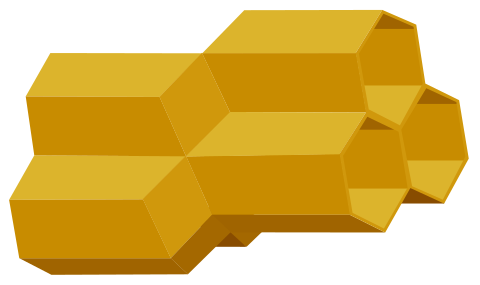
\includegraphics[width=\textwidth, height=0.2\textheight, keepaspectratio]
{res/honeycomb.png}
\caption{Dạng hình học của các ô tổ ong.}
\end{figure}
\end{frame}

\begin{frame}{Giải thuật tiến hóa (Evolutionary Algorithms)}
  Trước đây, con người huấn luyện các loài động vật thông qua thưởng hoặc
phạt, một việc làm ảnh hưởng trực tiếp đến độ khoẻ mạnh của cá thể, nhưng nếu
như bây giờ, ta có thể làm quá trình này hiệu quả hơn rất nhiều: bằng cách
\textbf{mô phỏng} lại quá trình này trong máy tính.

  Tuy nhiên, chúng ta không thể làm một mô phỏng chính xác 100\%
như với thực tế, mà chỉ có thể \textbf{chọn lọc các tính năng muốn mô phỏng}, và
\textbf{thực hiện các phép xấp xỉ phù hợp}. Mỗi cách này cho ta một thuật toán,
nằm trong lớp các \textbf{giải thuật tiến hóa}.

\begin{figure}
  \centering
  
\includegraphics[width=0.8\textwidth, height=0.2\textheight,
  keepaspectratio]{res/hdd.jpg}
\captionsetup{justification=centering,margin=2.5cm}
  \caption{Người ta ước tính, để lưu lượng thông tin của
  các nguyên tử trong một ổ đĩa sẽ cần $10^{12}$ ổ đĩa như thế.}
\end{figure}
\end{frame}

% subsection Giải thuật tiến hóa (Evolutionary Algorithms) (end)

\subsection{Các khái niệm chung của các giải thuật tiến hóa} % (fold)
\label{sub:Các khái niệm chung của các giải thuật tiến hóa}

\begin{frame}{Hàm fitness và hàm mục tiêu}
Như đã nói ở phần trên, các giải thuật tiến hóa thực hiện mô phỏng lại quá trình
sống của các cá thể có trong tự nhiên. Các cá thể sẽ, một cách tự nhiên, 
sinh sản và tạo ra các cá thể khỏe mạnh hơn, và nhờ đó tiến hóa.

Do vậy, nếu ta đánh giá sự khỏe mạnh của một cá thể bằng một ánh xạ $f: P \to
\mathbb{R}$, từ $P$: tập các cá thể hợp lệ cho đến tập số thực, thì quá
trình trên sẽ làm tiến hóa các cá thể của nó làm tối đa $f$, giúp cho người dùng
thu được một nghiệm (có thể) tối ưu của hàm mục tiêu $f$.

$f$ ở đây, ngoài cách gọi là hàm mục tiêu (objective function) trong Toán tối ưu
(Mathemetical Optimization), trong các giải thuật tiến hóa còn được gọi là "hàm
độ khỏe mạnh"\footnote
{Thuật ngữ này không được sử dụng nhiều trong tiềng Việt,
nhưng thuật ngữ tương ứng trong tiếng Anh được sử dụng tương đối nhiều.} hay 
\textbf{hàm fitness} (fitness function), do tính liên quan mật thiết giữa $f$
với độ khoẻ mạnh của cá thể.

\end{frame}

\begin{frame}{Hàm fitness và hàm mục tiêu}
Giữa toán tối ưu và giải thuật tiến hóa có một sự bất đồng nho nhỏ như sau: các
bài toán tối ưu thường được phát biểu dưới dạng bài toán min, nhưng các giải
thuật tiến hóa sẽ làm tối đa hàm fitness. Do đó, có nhiều trường hợp mà ta không
tối đa hóa hàm fitness mà lại tối thiểu hóa nó.

\begin{figure}
\centering
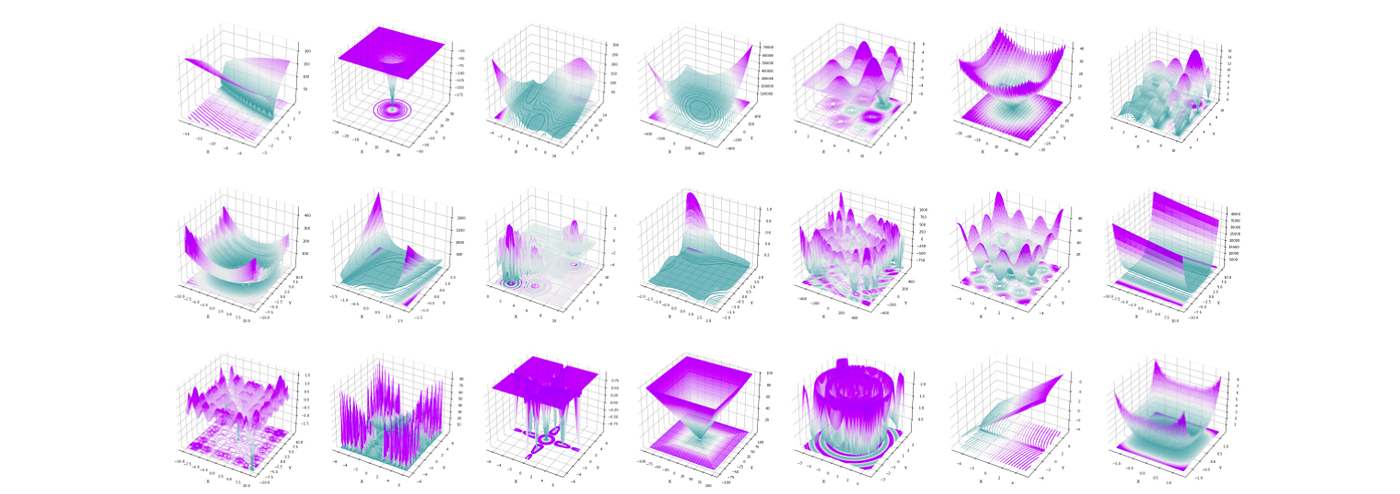
\includegraphics[width=\textwidth, height=0.5\textheight, keepaspectratio]
{res/discrep.png}
\captionsetup{justification=centering,margin=3cm}
\caption{Đồ thị hàm mục tiêu của các bài toán thử, thường được phát biểu dưới
dạng bài toán tìm min.}
\end{figure}
\end{frame}

\begin{frame}{Mã hóa cá thể}
Ở phần này, ta sẽ làm rõ hơn về cá thể. Về lý thuyết, cá thể trong giải thuật
tiến hóa có thể là bất cứ thứ gì, miễn là nó có khả năng sinh sản.

Tuy nhiên, lấy ý tưởng từ cách thông tin di truyền được lưu trữ trong ADN của
sinh vật dưới dạng hai chuỗi các nucleotide, người ta thường lấy dạng biểu diễn
của một ADN là một mảng kích thước định sẵn, thường là một mảng số nguyên hoặc
một mảng số thực. Mảng này được gọi là một \textbf{nhiễm sắc thể} (chromosome),
và các phần tử của nó là các \textbf{gen} (gene).

Vì thế, nảy sinh ra một vấn đề: ta cần một cách \textbf{mã hóa} một cá thể bất
kì: từ $P$ - tập các cá thể, sang $C$ - tập các nhiễm sắc thể, và ngược lại:
\begin{align*}
  \operatorname{encode}&: P \to C \\
  \operatorname{decode} &: C \to P \\
.\end{align*}
\end{frame}


\begin{frame}[fragile]
\frametitle{Mã hóa cá thể}
Với cá thể là các vector trong \( \mathbb{R}^{n} \) thì quá trình mã hóa có thể
chỉ đơn thuần là giữ nguyên vector này, nhưng trong thực tế, giữ nguyên vector
sẽ nảy sinh ra nhiều vấn đề cho tối ưu đa nhiệm. Ta sẽ xử lý vấn đề này sau khi
ta đi đến phần tiến hóa đa nhiệm.

Với cá thể có dạng phức tạp hơn, ta sẽ phải có các phương pháp mã hóa thích hợp
cụ thể. Chẳng hạn với một đường đi (hoặc chu trình) Hamilton (đi qua mọi đỉnh của đồ
thị) có thể được mã hóa dưới một mảng lưu thứ tự đi qua các đỉnh (các đỉnh của
đồ thị được đánh số).

Tuy nhiên ở đây, ta thấy rằng không phải một mảng chỉ mã hóa cho một đường đi
như vậy khi các phần tử của mảng đều đôi một khác nhau. Nghĩa là, một mảng không
thỏa mãn điều kiện này không phải là một nhiễm sắc thể đối với cách mã hóa trên.
\end{frame}

\begin{frame}{Các toán tử di truyền}
  Trong các giải thuật tiến hóa, các \textbf{toán tử di truyền} là các toán tử
  được sử dụng để làm cho quần thể ngày càng tối ưu hơn. Nó chính là những sự mô
  phỏng lại các quá trình có trong thực tế.

  Một toán tử di truyền quan trọng là \textbf{toán tử sinh sản}, được lấy ý tưởng từ
  quá trình sinh sản trong tự nhiên có hai loại chính: sinh sản vô tính và sinh
  sản hữu tính. Sinh sản vô tính chỉ cần một cá thể cha mẹ, nhưng sinh sản hữu
  tính cần hai (và hai cá thể này phải khác giới).

  Tổng quát lên, các toán tử sinh sản trong các giải thuật tiến hóa có thể cần
  đến một,  hai, hoặc nhiều hơn các cá thể cha mẹ, và có thể sinh ra một, hai,
  hoặc nhiều hơn cá thể con. Toán tử sinh sản có nhiệm vụ quan trọng là tạo ra
  những cá thể mới, những cá thể con có thể tối ưu hơn các cá thể cha mẹ của nó.

  Toán tử sinh sản đảm bảo \textbf{tính kế thừa} trong ba tiêu chí để chọn lọc
  tự nhiên.
\end{frame}

\begin{frame}{Các toán tử di truyền}
  Toán tử sinh sản được thực hiện sẽ làm cho quần thể ngày càng đông đúc hơn,
  làm tốn bộ nhớ và khả năng tính toán. Các cá thể kém tối ưu cũng sẽ có nhiều
  khả năng sinh sản ra những cá thể con cũng kém tối ưu, làm thuật toán kém hiệu
  quả đi nhiều lần.

  Chính vì vậy, cần có một toán tử để làm mất đi các cá thể cũ, đặc biệt là các
  cá thể có fitness thấp. Tuy nhiên, vẫn nên giữ lại một số những cá thể này để
  làm đa dạng quần thể, giúp cho quần thể không bị mắc kẹt ở một điểm tối ưu địa
  phương.

  Toán tử này chính là \textbf{toán tử chọn lọc}. Nó là nguyên nhân chính
  làm cho quần thể càng ngày càng tối ưu hơn. Một cách cài đặt đơn giản của toán
  tử này được là thông qua loại bỏ mọi cá thể nằm ngoài top $N$ của quần thể
  theo độ tối ưu, với $N$ là số lượng cá thể trước sinh sản.

  Toán tử sinh sản đảm bảo \textbf{tính chọn lọc} trong ba điều kiện của chọn
  lọc tự nhiên.
\end{frame}

\begin{frame}[fragile]
\frametitle{Thế hệ}

Sau các toán tử sinh sản và chọn lọc, quần thể nói chung đã trở nên tối ưu so
với quần thể ban đầu. Nếu toán tử của ta không loại bỏ các cá thể khỏe mạnh từ
quần thể ban đầu, thì các cá thể đó sẽ sống lâu cho đến khi nó bị loại bỏ do
toán tử chọn lọc, nghĩa là có các
cá thể tối ưu hơn nó. Do vậy, trong trường hợp này, quần thể sẽ luôn tối ưu hơn
quần thể trước nó.

Bằng cách lặp đi lặp lại các toán tử trên, ta thu được một quần thể ngày càng
tối ưu hơn. Mỗi bước lặp này gọi là một \textbf{thế hệ}.

\begin{minted}{python}
def basic_ea():
  while True:
    # trong mỗi thế hệ
    reproduce(population) # thực hiện sinh sản
    selection(population) # thực hiện chọn loc
    yield population # trả lại quần thể sau mỗi bước lặp
\end{minted}
\end{frame}

% subsection Các khái niệm chung của các giải thuật tiến hóa (end)

\subsection{Đánh giá chung các giải thuật tiến hóa} % (fold)
\label{sub:Đánh giá chung các giải thuật tiến hóa}

\begin{frame}{Đánh giá chung các giải thuật tiến hóa}
Đầu tiên, giải thuật tiến hóa (nói chung) có thể được áp dụng cho hầu hết các loại bài toán tối ưu như quy hoạch phi tuyến, quy hoạch nguyên hay tối ưu tổ hợp.

Các giải thuật tiến hóa không có đòi hỏi gì quá đặc biệt đối với hàm mục tiêu và
miền nghiệm, nó không cần tính khả vi như phương pháp hướng giảm gradient hoặc
phương pháp Newton, nên vô cùng phù hợp đối với các bài toán rời rạc.

Do đó, giải thuật tiến hóa không đòi hỏi ở người cài đặt thuật toán nhiều, mà chỉ
cần hiểu cách thuật toán hoạt động là đủ. Việc thay thế hàm mục tiêu cũng rất
đơn giản do giải thuật không sử dụng tính chất đặc biệt gì của hàm này.

Tuy nhiên, một hàm mục tiêu quá đơn giản như sau:
\[
  f(x) = 
  \begin{cases}
    1, &\text{nếu } x = 0 \\
    0, &\text{nếu ngược lại}
  \end{cases}
,\]  làm mất đi khả năng đánh giá tính tốt kém của các
cá thể, khi hầu hết các cá thể đều tốt như nhau, sẽ khiến cho giải thuật tiến
hóa không hiệu quả.
\end{frame}

\begin{frame}{Đánh giá chung các giải thuật tiến hóa}
  Tuy nhiên, do lượng thông tin ít ỏi mà giải thuật được cung cấp, nên ta sẽ
  không chắc chắn được gì nhiều về kết quả của thuật toán. Với các giải thuật
  elitist, nếu ít nhất cá thể tốt nhất của mỗi thế hệ được giữ lại, thì sự hội
  tụ là chắc chắn, nhưng chưa chắc là điểm hội tụ là nghiệm tối ưu toàn cục.

  Các đặc điểm của sự hội tụ này, như tốc độ hội tụ của nghiệm và giá trị hàm
  mục tiêu, cũng không thể được suy ra như ở các thuật toán khác.

  Điều kiện dừng của các giải thuật tiến hóa cũng không rõ ràng. Cá thể trong
  quần thể là có thể là nghiệm tối ưu toàn cục, nhưng giải thuật nói chung không
  có cách nào để chắc chắn tính tối ưu này của nghiệm.
\end{frame}

% subsection Đánh giá chung các giải thuật tiến hóa (end)


% section Ứng dụng các cơ chế tiến hóa trong tối ưu (end)
